\chapter{Evaluation}
\label{evaluation}
\nocite{*}

In diesem Kapitel werden die Ergebnisse der Untersuchung der Large Language Models (\acp{LLM}) und Embedding-Modelle umfassend dargestellt und ausgewertet. 

Die Ergebnisse dieser Untersuchung bilden die Grundlage für die abschließende Entscheidung zur Auswahl der geeigneten Modelle und dienen als Referenz für die technische Umsetzung im nachfolgenden Abschnitt.

\section{Evaluation Large Language Modellen}
\label{eval_llm}

Im Rahmen der Entwicklung eines \ac{KI}-basierten Chatbots für Freudenberg \& Co. KG (\ac{FCO}) wurde, basierend auf dem in Abschnitt \ref{eval_llm_konzept} vorgestellten Untersuchungskonzept, 
eine umfassende Untersuchung verschiedener Large Language Models (\acp{LLM}) durchgeführt, die auf SAP AI Core innerhalb der SAP Business Technology Platform (\ac{BTP}) verfügbar sind. 
Da diese Modelle für die geplante Implementierung des Chatbots relevant sind, konzentriert sich die Untersuchung auf die in SAP AI Core angebotenen Modelle, 
um eine fundierte Entscheidung für die spezifischen Anforderungen des Projekts treffen zu können.

Die getesteten Modelle umfassen die Open-Source-Modelle \textit{LLaMA3-70b}, \textit{Mistral-8x7b}, \textit{Falcon-40b} sowie die Modelle \textit{GPT-3.5-Turbo} und \textit{GPT-4o} von OpenAI. 
Jedes Modell wurde unter verschiedenen Konfigurationen evaluiert, wobei \textit{chunk sizes} von 64, 128, 256 und 512 getestet wurden. Zudem wurden die \textit{top k}-Werte 4, 6, 8, 10, 15 und 20 verwendet, 
um die Anzahl der in den Kontext einbezogenen Antworten zu variieren. Dies führte insgesamt zu 24 Konfigurationen pro Modell, was eine umfassende und detaillierte Bewertung der Leistungsfähigkeit ermöglicht.

Für jede Konfiguration wurden 100 Prompts durchgeführt, die auf 10 deutsche und 10 englische Dokumente verteilt waren. Die Ergebnisse für jedes \ac{LLM} wurden gespeichert, 
um eine genaue Analyse der Leistung unter den verschiedenen Konfigurationen zu ermöglichen. Anschließend wurde der Durchschnitt der Ergebnisse pro Konfiguration und Modell berechnet, 
um eine Vergleichbarkeit zu gewährleisten und präzise Aussagen darüber treffen zu können, wie die einzelnen \acp{LLM} bei jeder Konfiguration performen.

Die Vielzahl der getesteten Parameter gewährleistet, dass die Modelle auf einer breiten Datenbasis evaluiert werden, um präzise Rückschlüsse auf ihre Leistungsfähigkeit zu ziehen. 
Darüber hinaus hilft diese Untersuchung dabei, die optimalen Parameterkonfigurationen für den praktischen Einsatz im Chatbot zu bestimmen.

Die Evaluation erfolgt unter Berücksichtigung der Kriterien Antwortqualität, Antwortzeit und Kosten. Diese Kriterien stellen sicher, dass das ausgewählte Modell nicht nur qualitativ hochwertige und relevante Antworten liefert, 
sondern auch effizient und kostengünstig in Echtzeitanwendungen integriert werden kann.

In den folgenden Abschnitten werden die Ergebnisse der Evaluation detailliert analysiert und die Leistung der Modelle miteinander verglichen.

\subsection{Antwortqualität}

Die Antwortqualität der verschiedenen \acp{LLM} wurde anhand einer normalisierten Bewertungsfunktion \ref{eq:score_function_quali} ermittelt. 
Hierbei wurde der Ähnlichkeitsscore, den \textit{GPT-3.5-Turbo} für jede generierte Antwort in Bezug auf eine perfekte Antwort vergeben hat, 
auf eine Skala von 0 bis 1 normalisiert und anschließend mit einem Faktor von 10 multipliziert. 
Dies ermöglicht eine einheitliche Bewertung der Antwortqualität auf einer Skala von 0 bis 10, wobei 10 die höchste Übereinstimmung mit der perfekten Antwort darstellt.

Diese Normalisierung stellt sicher, dass die Bewertung der Antwortqualität für alle Modelle konsistent und vergleichbar bleibt. 
Sie minimiert Verzerrungen und garantiert, dass die Modelle im Verhältnis zu ihrer maximal erreichbaren Leistung bewertet werden.

\begin{equation}
    \mbox{Score Function} = \mbox{gpt-3.5-turbo\_judgement} \cdot 10
    \label{eq:score_function_quali}
\end{equation}

In Abbildung \ref{fig:antwortqualität} sind die Ergebnisse der Antwortqualität in Form eines Streudiagramms dargestellt. 
Auf der X-Achse sind die unterschiedlichen Konfigurationen von \textit{chunk size} und \textit{top k} abgetragen, während die Y-Achse den Antwort-Score von 0 bis 10 wiedergibt.
Die Modelle \textit{GPT-4o}, \textit{GPT-3.5-Turbo} und \textit{LLaMA3-70b} erreichen konsistent hohe Scores, was ihre Fähigkeit zur präzisen und relevanten Beantwortung komplexer Anfragen unterstreicht.
\textit{GPT-4o} zeigt hierbei in den meisten Konfigurationen die höchsten Scores, was seine besondere Eignung für die präzise Bearbeitung anspruchsvoller Anfragen hervorhebt.
Im Gegensatz dazu erzielt \textit{Falcon-40b} durchgehend niedrigere Scores, was auf eine geringere semantische Präzision und Genauigkeit seiner Antworten schließen lässt.

\begin{figure}[H]
    \centering
    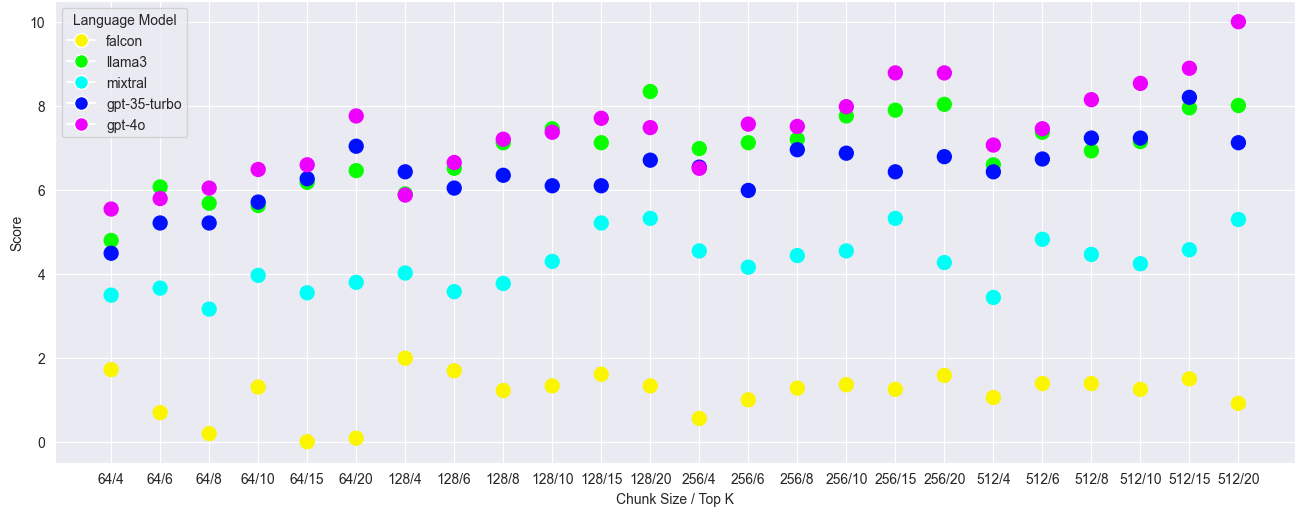
\includegraphics[width=1\textwidth]{img/antwortquali.png}
    \caption{Antwortqualität Untersuchung \acp{LLM}}
    \label{fig:antwortqualität}
\end{figure}

\subsection{Antwortzeit}

Die Antwortzeit stellt ein zentrales Kriterium für die Praktikabilität von \acp{LLM} in Echtzeitanwendungen dar. Um diese zu bewerten, wurde die Laufzeit für jede Anfrage gemessen, beginnend mit dem Zeitpunkt des Absendens eines Prompts bis zur Rückgabe der Antwort durch das Modell.
Anschließend wurde für jede Konfiguration der Durchschnitt der Laufzeiten berechnet.

Das berechnete Ergebnis wird in der Bewertungsfunktion \ref{eq:score_function_zeit} als Maß für die Effizienz der jeweiligen Konfiguration verwendet.

\begin{equation}
    \mbox{Score Function} = \mbox{avg\_runtime}
    \label{eq:score_function_zeit}
\end{equation}

Alle Tests wurden unter denselben Bedingungen in einem stabilen lokalen LAN-Netzwerk auf identischer Hardware durchgeführt. 
Diese kontrollierte Umgebung stellte sicher, dass die Laufzeiten der Modelle unter fairen und vergleichbaren Bedingungen ermittelt wurden.

In Abbildung \ref{fig:antwortzeit} sind die durchschnittlichen Antwortzeiten der Modelle als Streudiagramm dargestellt. 
Auf der X-Achse sind die unterschiedlichen Konfigurationen von \textit{chunk size} und \textit{top k} dargestellt, während die Y-Achse die Antwortzeit (Runtime) in Millisekunden wiedergibt. 
Die Werte reichen hierbei von unter 1000 ms bis knapp unter 9000 ms.
Modelle wie \textit{GPT-4o} und \textit{GPT-3.5-Turbo} verzeichneten durchweg kurze Antwortzeiten, was sie besonders für den Einsatz in Echtzeitanwendungen prädestiniert. 
Im Gegensatz dazu zeigte das Modell \textit{Falcon-40b} signifikant längere Antwortzeiten, was dessen Einsatzpotenzial in zeitkritischen Szenarien deutlich einschränkt.

Die Unterschiede in der Antwortzeit lassen sich teilweise auf die Infrastrukturen zurückführen, die hinter den Modellen stehen. 
Modelle von OpenAI, wie \textit{GPT-4o} und \textit{GPT-3.5-Turbo}, profitieren von spezialisierter Hardware in hoch optimierten Rechenzentren, was ihre Geschwindigkeit verbessert. 
Open-Source-Modelle wie \textit{Falcon-40b} haben oft nicht denselben Zugang zu spezialisierten Infrastrukturen, was sich negativ auf ihre Laufzeiten auswirkt.

\begin{figure}[H]
    \centering
    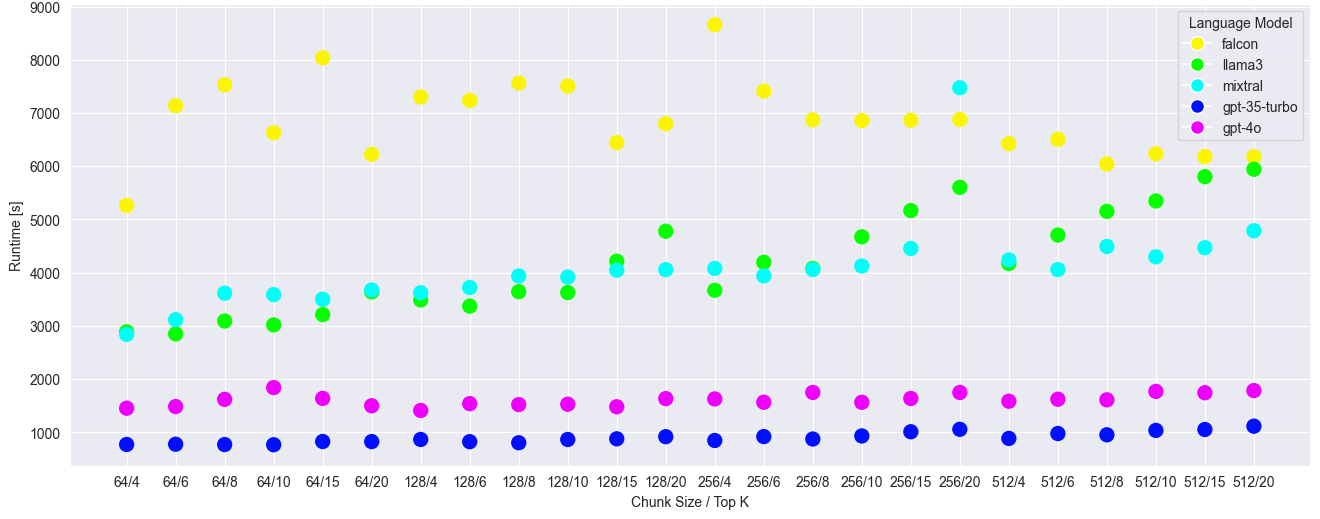
\includegraphics[width=1\textwidth]{img/antwortzeit.png}
    \caption{Antwortzeiten Untersuchung \acp{LLM}}
    \label{fig:antwortzeit}
\end{figure}

\subsection{Kosten}

Die Kostenbewertung der Large Language Models (\acp{LLM}) basiert auf der Messung des Tokenverbrauchs pro Anfrage. 
Der Tokenverbrauch wurde bei jedem Untersuchungslauf gemessen, wobei für einige Modelle, wie \textit{GPT-4o} und \textit{GPT-3.5-Turbo}, der Tokenverbrauch direkt von den \acp{API} von SAP AI Core bereitgestellt wird. 
Für Modelle, die diese Information nicht nativ liefern, wie \textit{LLaMA3-70b}, wurde die Token-Anzahl mithilfe der Python-Library \textit{tokenizers} ermittelt. 
Dieses Tool ermöglicht eine präzise Berechnung des Tokenverbrauchs anhand der jeweiligen Tokenizer-Spezifikationen der Modelle. 
Die \textit{tokenizer.json}-Dateien für die entsprechenden Modelle wurden dabei von der Plattform Hugging Face heruntergeladen und verarbeitet.

Um die Gesamtkosten zu ermitteln, wurde der Tokenverbrauch für jeden Untersuchungslauf gemessen und mit den festgelegten Kosten für Input- und Output-Tokens der \acp{LLM}, wie sie von SAP AI Core vorgegeben sind, multipliziert. Um die Ergebnisse zu standardisieren, 
wurde in der Bewertungsfunktion \ref{eq:score_function_kosten} der normalisierte Durchschnitt mit einem Faktor von 10 multipliziert.

\begin{equation}
    \mbox{Score Function} = \mbox{avg\_cost} \cdot 10
    \label{eq:score_function_kosten}
\end{equation}

In Abbildung \ref{fig:kosten} sind die normalisierten Kosten pro Prompt für jede Konfiguration und jedes \ac{LLM} dargestellt. 
Die X-Achse zeigt die verschiedenen Konfigurationen hinsichtlich \textit{chunk size} und \textit{top k}, während die Y-Achse den Score von 0 bis 10 wiedergibt, wobei höhere Scores höhere Kosten anzeigen.

Die Ergebnisse verdeutlichen, dass \textit{GPT-4o} in allen Konfigurationen die höchsten Kosten verursacht, was auf den erhöhten Rechenaufwand und die Ressourcenanforderungen hinweist, 
die zur Generierung präziser und detaillierter Antworten benötigt werden. Im Gegensatz dazu sind die Kosten für \textit{Falcon-40b} und \textit{Mistral-8x7b} deutlich geringer, 
was diese Modelle insbesondere für kostensensitive Anwendungen interessant macht.



\begin{figure}[H]
    \centering
    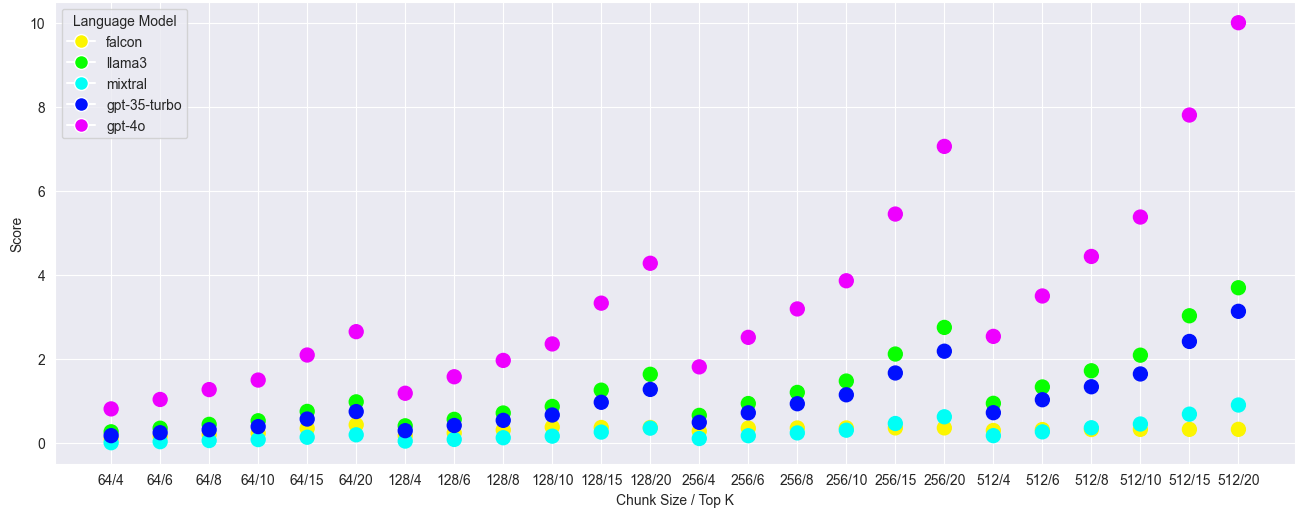
\includegraphics[width=1\textwidth]{img/kosten.png}
    \caption{Kosten Untersuchung \acp{LLM}}
    \label{fig:kosten}
\end{figure}

\subsection{Gesamtbewertung}

Die Gesamtbewertungsfunktion \ref{eq:score_function_gesamt} berücksichtigt drei Hauptkomponenten: die Qualität der Antworten, die Antwortzeit und die Gesamtkosten. 
Diese Faktoren werden mit unterschiedlichen Gewichtungen kombiniert, um eine umfassende Bewertung der Leistungsfähigkeit der Modelle zu ermöglichen.

\begin{equation}
    \mbox{Score Function} = \mbox{\textit{gpt\_judgement}} \cdot 10 - \mbox{\textit{avg\_runtime}} \cdot 2 - \mbox{\textit{total\_cost}} \cdot 5
    \label{eq:score_function_gesamt}
\end{equation}

Die \textit{gpt judgement}-Komponente bezieht sich auf die Bewertung der Antwortqualität, die durch \textit{GPT-3.5-Turbo} vorgenommen wurde. 
Die Antwortqualität wurde auf einer Skala von 0 bis 1 normalisiert und anschließend mit 10 multipliziert, um sie in den gleichen Wertebereich wie die anderen Faktoren zu skalieren. 
Die \textit{average runtime} wurde ebenfalls auf einer Skala von 0 bis 1 normalisiert, um sicherzustellen, dass die Laufzeitfaktoren vergleichbar verrechnet werden können. 
Die \textit{total cost}-Komponente umfasst die Gesamtkosten, die mit jedem Prompt verbunden sind, und wurde ebenfalls auf einer Skala von 0 bis 1 normalisiert, 
um die finanzielle Effizienz der Modelle in Bezug auf deren Leistungsfähigkeit zu bewerten.

Die Gewichtung der Antwortzeit mit dem Faktor 2 und der Kosten mit dem Faktor 5 in der Score Function \ref{eq:score_function_gesamt} basiert auf den Ergebnissen einer internen Umfrage unter Testnutzern, 
wie im Untersuchungskonzept \ref{eval_llm_konzept} beschrieben. Diese Umfrage erfasste die Prioritäten der Testnutzer hinsichtlich Antwortgeschwindigkeit und Kosten, 
während die Antwortqualität als das wichtigste Kriterium festgelegt und mit einem Faktor von 10 gewichtet wurde.

Leider trat während der Sicherung der Umfrageergebnisse ein Fehler im Backup-Prozess auf, der dazu führte, dass die Rohdaten irreversibel verloren gingen. 
Jedoch wurden die Umfrageergebnisse zuvor in einer Excel-Datei gesichert, was die Berechnung von Mittelwert und Median ermöglichte, sodass diese Kennzahlen weiterhin zur Verfügung stehen.

In Abbildung \ref{fig:prioritäten} sind die Antworten der Umfrage visualisiert. 
Für die Antwortgeschwindigkeit ergab sich ein Mittelwert von 2,09 und ein Median von 2, was darauf hindeutet, dass Geschwindigkeit als relevant, aber nicht als primäres Kriterium angesehen wird. 
Im Gegensatz dazu zeigt das Ergebnis für die Kosten einen Mittelwert von 4,55 und einen Median von 5, was die hohe Bedeutung der Kosten für die Testnutzer verdeutlicht.

\begin{figure}[H]
    \centering
    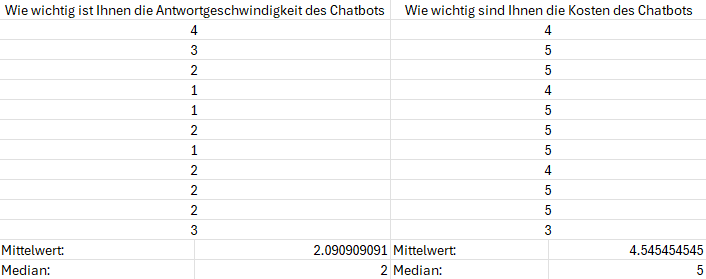
\includegraphics[width=0.8\textwidth]{img/prioritaeten.png}
    \caption{Prioritäten der Testnutzer in Bezug auf Antwortgeschwindigkeit und Kosten}
    \label{fig:prioritäten}
\end{figure}

Diese Umfrageergebnisse wurden herangezogen, um die Gewichtungen der \textit{avg runtime} und \textit{total cost} in der Score Function \ref{eq:score_function_gesamt} zu bestimmen. 
Dadurch wird gewährleistet, dass Modelle, die qualitativ hochwertige Antworten liefern, gleichzeitig effizient in der Laufzeit und kostengünstig sind, 
die höchste Gesamtbewertung erzielen. Die Score Function ermöglicht somit eine ausgewogene Berücksichtigung aller relevanten Faktoren und unterstützt eine fundierte Entscheidungsfindung bei der Auswahl der geeignetsten Modelle.

In Abbildung \ref{fig:gesamtwert} sind die Ergebnisse der Gesamtbewertung der Modelle dargestellt. 
Die Modelle \textit{GPT-4o}, \textit{GPT-3.5-Turbo} und \textit{LLaMA3-70b} erreichten hierbei die höchsten Scores, was auf ihre gute Balance zwischen Antwortqualität, Antwortzeit und Kosten hinweist. 
\textit{Falcon-40b} hingegen erzielte aufgrund seiner geringeren Antwortqualität und längeren Antwortzeiten eine vergleichsweise niedrige Gesamtbewertung.

\begin{figure}[H]
    \centering
    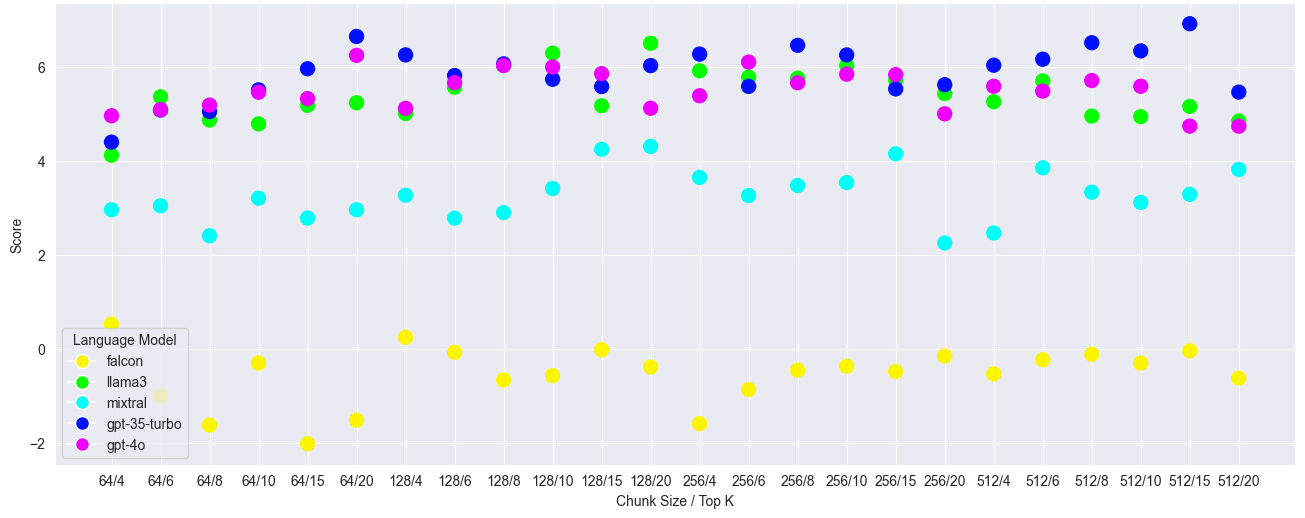
\includegraphics[width=1\textwidth]{img/gesamtScore.png}
    \caption{Gesamtbewertung der Untersuchung der \acp{LLM}}
    \label{fig:gesamtwert}
\end{figure}

Auf Basis dieser Ergebnisse lässt sich festhalten, dass \textit{LLaMA3-70b} das beste Open-Source-Modell darstellt, während \textit{GPT-3.5-Turbo} in der Gesamtbewertung die besten Leistungen erbringt. 
Sollte in der Score Function \ref{eq:score_function_gesamt} die Gewichtung der Kosten reduziert oder entfernt werden, wäre \textit{GPT-4o} das leistungsstärkste Modell.

Die Ergebnisse dieser Evaluation bieten eine solide Grundlage für die Auswahl der am besten geeigneten Modelle, um den spezifischen Anforderungen der Freudenberg Gruppe gerecht zu werden. 
Wenn Open-Source-Anforderungen bestehen, ist \textit{LLaMA3-70b} die beste Wahl. Sollte das Budget keine Rolle spielen, empfiehlt sich \textit{GPT-4o}. 
Andernfalls stellt \textit{GPT-3.5-Turbo} die effizienteste Option dar.

\section{Evaluation von Embedding Modellen}
\label{eval_embedding}

Die Untersuchung der Embedding-Modelle basiert auf dem in Abschnitt \ref{eval_embedding_konzept} beschriebenen Konzept. Ziel der Evaluation war es, die semantische Leistungsfähigkeit der Modelle zu bewerten, 
insbesondere in Bezug auf die Fähigkeit, relevante Textabschnitte in großen Dokumenten korrekt zu identifizieren und zu ordnen. 
Die Modelle, die auf der SAP \ac{BTP} verfügbar sind und in die Evaluation einbezogen wurden, umfassen \textit{multilingual-e5-large}, ein Open-Source-Modell, 
sowie das Modell \textit{ada-Embeddings} und das neuere \textit{text-embedding-3-large} von OpenAI. Diese Modelle wurden aufgrund ihrer Verfügbarkeit und Relevanz für die geplante Implementierung des Chatbots ausgewählt.

Die Leistungsbewertung der Modelle erfolgte anhand der Metriken Mean Reciprocal Rank (\ac{MRR}) und Precision at k. Der \ac{MRR} misst, wie hoch die korrekte Antwort in der Ergebnisliste eines Modells platziert wird, 
wobei ein hoher \ac{MRR}-Wert auf eine hohe Genauigkeit bei der Platzierung relevanter Textstellen hinweist. Zusätzlich bewertet Precision at k, wie viele der zurückgegebenen Ergebnisse tatsächlich relevant sind, 
was die Effizienz der Modelle in der Erkennung relevanter Abschnitte reflektiert.

Die Performanz in Bezug auf Antwortgeschwindigkeit und Ressourcenverbrauch wurde nicht separat untersucht, da die Unterschiede zwischen den Embedding-Modellen in diesen Bereichen marginal waren. 
Das Embedden von Dokumenten spielt im gesamten \ac{RAG}-Prozess eine untergeordnete Rolle, da der Großteil der Verarbeitungszeit durch den \ac{LLM}-Call bestimmt wird.

Die Ergebnisse zeigten, dass das Open-Source-Embedding-Modell \textit{multilingual-e5-large} im Vergleich zu den \textit{ada-Embeddings} von OpenAI leicht überlegen war. 
Das beste Ergebnis wurde jedoch durch das neuere Modell \textit{text-embedding-3-large} von OpenAI erzielt. Dieses Modell war in der Lage, häufiger relevante Chunks in den oberen Rängen der Ergebnisliste zu platzieren, 
was zu höheren Werten in den Metriken \ac{MRR} und Precision at k führte. Obwohl die Unterschiede zwischen den Modellen insgesamt gering waren, 
konnte \textit{text-embedding-3-large} in vielen Fällen mehr relevante Textabschnitte erkennen und platzieren.

Leider können in dieser Arbeit keine detaillierten Werte zu den Embedding-Modellen dargestellt werden, da die Testergebnisse der Embeddings nur im Vergleich zueinander gespeichert wurden, 
ohne spezifische \ac{MRR}- oder Precision at k-Werte zu archivieren. Während die \ac{LLM}-Ergebnisse vollständig gesichert wurden, 
beschränkte sich die Dokumentation der Embedding-Modelle auf qualitative Vergleiche. Der Zugriff auf den Laptop, auf dem die Versuche durchgeführt wurden, 
ist inzwischen nicht mehr möglich, weshalb keine genauen Zahlenwerte für diese Evaluation nachträglich abrufbar sind.
